\ylDisplay{Rong} % Ülesande nimi
{Tundmatu autor} % Autor
{lahtine} % Voor
{2006} % Aasta
{G 10} % Ülesande nr.
{9} % Raskustase
{
% Teema: Dünaamika
\ifStatement
Rong sõidab kiirusega $v = \SI{100}{km/h}$ ja pidurdab järsult (blokeerides rattad). Graafikul on toodud rongi rataste ja rööbaste vahelise hõõrdeteguri $\mu$ sõltuvus kiirusest (\si{km/h}).\\
\osa Kui pikk on rongi täieliku peatumiseni kulunud aeg?\\
\osa Kui suur on pidurdusmaa pikkus? Mõlemad vastused tuleb leida
graafikualuste pindaladena sobilikult valitud teljestikes.

\begin{center}
	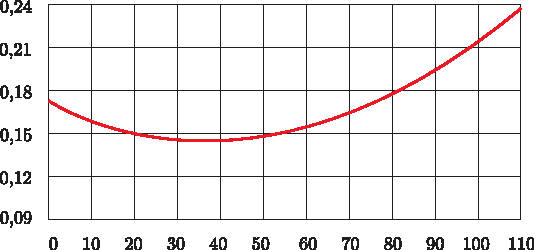
\includegraphics[width=\linewidth]{2006-lahg-10-yl}
\end{center}
\fi


\ifHint
Otsitavate suuruste jaoks on kasulik vaadelda lühikest ajavahemikku $\Delta t$, mille jooksul on rongi kiirus, ja seega hõõrdetegur, ligikaudu konstantsed. Seejärel saab saadud ajavahemikke summeerida terve graafiku ulatuses. Selle jaoks peab vajadusel konstrueerima uued graafikud teistsuguste telgedega.
\fi


\ifSolution
\osa Vaatame väikest kiiruste vahemikku $\Delta v$, mille sees võib kiirust $v$ ja järelikult ka hõõrdetegurit $\mu (v)$ lugeda konstantseks. Kiirendus on selle liikumisfaasi jooksul siis $a = \mu (v)g$ ning kiiruse vähenemiseks kuuluv aeg
\[
\Delta t=\frac{\Delta v}{a}=\frac{\Delta v}{\mu(v) g}.
\]

\begin{center}
	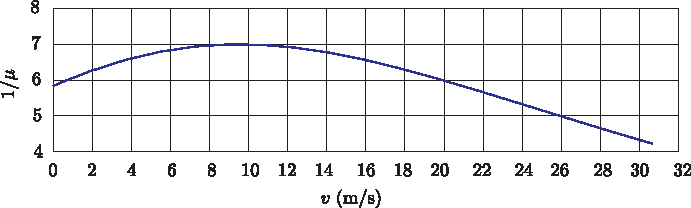
\includegraphics[width=\linewidth]{2006-lahg-10-lah1}
\end{center}

Summaarne aeg oleks summa üle kõigi selliste väikeste kiirusemuutuste. Konstrueerime esialgsest graafikust lähtudes suuruse $1/\mu (v)$ sõltuvuse kiirusest $v$ (vt joonist). Siis pidurdamiseks kuuluv aeg on selle sõltuvuse graafikualune pindala (kiirusest \num{0} kuni \SI{100}{km/h}), jagatud $g$-ga. Seejuures peame silmas, et kiirus $x$-teljel peab olema meetrites sekundis (\si{m/s}). Vastuseks saame ligikaudselt \SI{18}{s}.

\osa Vaatame samasugust kiiruste vahemikku $\Delta v$, nagu esimeses osas. Ajaga $\Delta t$ mille jooksul kiirus selle võrra väheneb, läbib rong teepikkuse
\[
\Delta s = v\Delta t = \frac{v\Delta v}{\mu (v)g}.
\]
Summaarne pidurdusmaa oleks summa üle kõigi selliste väikeste teepikkuste. Konstrueerime esialgsest graafikust lähtudes suuruse $v/\mu (v)$ sõltuvuse kiirusest $v$ (vt joonist). Siis pidurdusmaa on selle sõltuvuse graafikualune pindala (kiirusest \num{0} kuni \SI{100}{km/h}), jagatud $g$-ga. Kiirus $x$-teljel on samuti meetrites sekundis (\si{m/s}). Vastuseks saame ligikaudselt \SI{235}{m}.

\begin{center}
	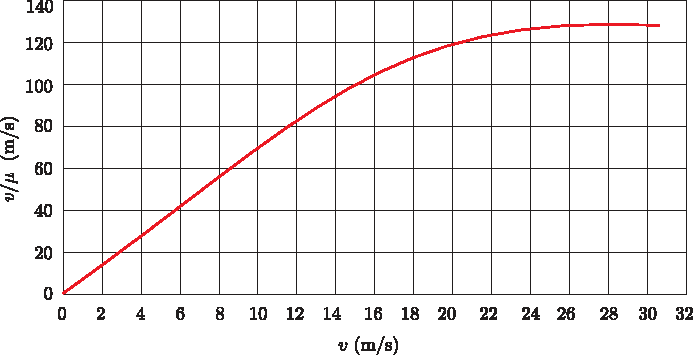
\includegraphics[width=\linewidth]{2006-lahg-10-lah2}
\end{center}

\emph{Märkus}. Integraalne avaldis pidurdusaja jaoks on kujul
\[
t=\int_{0}^{v_{0}} \frac{\D v}{\mu(v) g}=\frac{1}{g} \int_{0}^{v_{0}} \frac{\D v}{\mu(v)},
\]
kus $v_0$ on rongi algkiirus. Pidurdusmaa pikkuse jaoks vastav avaldis on aga
\[
s=\int_{0}^{v_{0}} \frac{v \D v}{\mu(v) g}=\frac{1}{g} \int_{0}^{v_{0}} \frac{v \D v}{\mu(v)}.
\]
\fi
}